% =============================================================================
%  Exosuit Cable Stiffness Control and Co-Contraction Mechanism
%  Addresses: coupling between joint rotation and stiffness modulation
% =============================================================================

\documentclass[11pt, a4paper]{article}

\usepackage{amsmath, amssymb, bm}
\usepackage{geometry}
\usepackage{hyperref}
\usepackage{booktabs}
\usepackage{xcolor}
\usepackage{graphicx}
\usepackage{tikz}
\usetikzlibrary{arrows.meta, decorations.pathmorphing, positioning, calc, patterns}
\usepackage{cleveref}
\usepackage[backgroundcolor=blue!5, linecolor=blue!40, linewidth=1pt,
            innertopmargin=6pt, innerbottommargin=6pt,
            innerleftmargin=7pt, innerrightmargin=7pt]{mdframed}

\geometry{margin=2.2cm}

% ── Standard project macros ──────────────────────────────────────────────────
\newcommand{\bq}{\bm{q}}
\newcommand{\bp}{\bm{p}}
\newcommand{\bu}{\bm{u}}
\newcommand{\btau}{\bm{\tau}}
\newcommand{\bF}{\bm{F}}
\newcommand{\bJ}{\bm{J}}
\newcommand{\bM}{\bm{M}}
\newcommand{\bC}{\bm{C}}
\newcommand{\bG}{\bm{G}}

\title{\textbf{Exosuit Cable Stiffness Control \\and Co-Contraction Mechanism}\\
       \large \texttt{cable/cable\_with\_exo\_springs.py}}
\date{April 2026}
\author{Isaac-sim robotics notes}

\begin{document}
\maketitle

% ═════════════════════════════════════════════════════════════════════════════
\section{Problem: Link~2 Strikes an Object}
\label{sec:problem}
% ═════════════════════════════════════════════════════════════════════════════

The cup manipulator's elbow joint~$q_2$ is driven by antagonistic
\textbf{drive cables} (green/red) via an SEA motor.  During normal
operation the drive cables alone govern joint motion:
%
\begin{equation}\label{eq:eom-drive}
    \bM(\bq)\,\ddot{\bq} + \bC(\bq,\dot{\bq})\,\dot{\bq} + \bG(\bq)
    = \begin{bmatrix} 0 \\ \tau_2^{\text{drive}} \end{bmatrix}.
\end{equation}

\noindent
\textbf{Scenario.}\;
The joint is at $q_2 = 30°\;(0.524\;\text{rad})$ when link~2 strikes an
object.  The impact deflects the joint to $q_2 = 45°$ --- a
$+15°\;(0.262\;\text{rad})$ disturbance.  The acceleration spike reaches
$|\ddot{q}_2| = 120\;\text{rad/s}^2$.

\medskip\noindent
\textbf{What we need:} increase the joint stiffness \emph{instantly} to
resist the deflection, without changing the equilibrium position.  The drive
cables cannot do this alone --- they are already committed to trajectory
tracking.

\medskip\noindent
\textbf{Solution:} a second set of cables --- the \textbf{exosuit cables}
(orange/magenta) --- that provide on-demand stiffness via co-contraction.
Two methods for routing these cables are compared in this document.

\begin{mdframed}
\textbf{Key design question (Thrish, April 2026):}
\emph{``Are the two purple motors driving only stiffness / co-contraction,
or are they driving the joint too?''}

\medskip\noindent
\textbf{Answer:} The exo motors drive \emph{only stiffness}.  The drive
cables actuate the joint.  Stiffness control is independent of and additive
to joint rotation control: when the exo motors are off, the springs are slack
and exert zero force regardless of~$q_2$.
\end{mdframed}


% ═════════════════════════════════════════════════════════════════════════════
\section{Physical Architecture}
\label{sec:architecture}
% ═════════════════════════════════════════════════════════════════════════════

\begin{figure}[h]
\centering
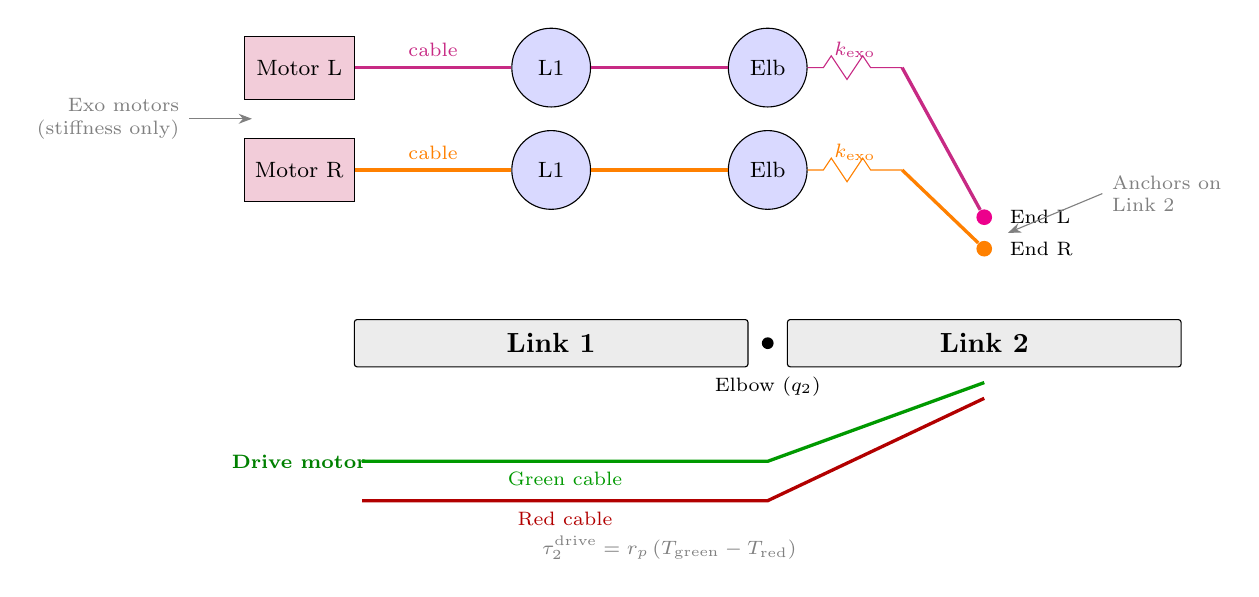
\begin{tikzpicture}[
    >=Stealth,
    pulley/.style={circle, draw, fill=blue!15, minimum size=10mm, font=\footnotesize},
    motor/.style={rectangle, draw, fill=purple!20, minimum width=14mm,
                  minimum height=8mm, font=\footnotesize},
    spring/.style={decorate, decoration={zigzag, segment length=4mm,
                   amplitude=1.5mm, pre length=2mm, post length=2mm}},
    cable/.style={very thick},
    link/.style={draw, fill=gray!15, minimum height=6mm, rounded corners=1pt},
]
    % ── Links ─────────────────────────────────────
    \node[link, minimum width=50mm] (link1) at (0,0) {\textbf{Link 1}};
    \node[link, minimum width=50mm] (link2) at (5.5,0) {\textbf{Link 2}};
    \node[fill=black, circle, inner sep=1.5pt] at (2.75,0) {};
    \node[below, font=\scriptsize] at (2.75,-0.3) {Elbow ($q_2$)};

    % ── Drive cable system (bottom) ──────────────
    \node[font=\scriptsize\bfseries, color=green!50!black] at (-3.2,-1.5) {Drive motor};
    \draw[cable, green!60!black] (-2.4,-1.5) -- node[below, font=\scriptsize, pos=0.5]
         {Green cable} (2.75,-1.5) -- (5.5,-0.5);
    \draw[cable, red!70!black]   (-2.4,-2.0) -- node[below, font=\scriptsize, pos=0.5]
         {Red cable}   (2.75,-2.0) -- (5.5,-0.7);
    \node[font=\scriptsize, color=gray] at (1.5,-2.6) {%
      $\tau_2^{\text{drive}} = r_p\,(T_{\text{green}} - T_{\text{red}})$};

    % ── Exo cable system (top) ────────────────────
    % Right exo cable (orange)
    \node[motor] (motorR) at (-3.2, 2.2) {Motor R};
    \node[pulley] (link1pR) at (0, 2.2) {L1};
    \node[pulley] (elbowpR) at (2.75, 2.2) {Elb};
    \node[circle, fill=orange, inner sep=2pt] (endR) at (5.5, 1.2) {};
    \node[right, font=\scriptsize] at (5.7, 1.2) {End R};

    \draw[cable, orange]  (motorR.east) -- node[above, font=\scriptsize] {cable}
                          (link1pR.west);
    \draw[cable, orange]  (link1pR.east) -- (elbowpR.west);
    \draw[spring, orange] (elbowpR.east) -- node[above, font=\scriptsize]
         {$k_{\text{exo}}$} ++(1.2,0) coordinate (spR);
    \draw[cable, orange]  (spR) -- (endR);

    % Left exo cable (magenta)
    \node[motor] (motorL) at (-3.2, 3.5) {Motor L};
    \node[pulley] (link1pL) at (0, 3.5) {L1};
    \node[pulley] (elbowpL) at (2.75, 3.5) {Elb};
    \node[circle, fill=magenta, inner sep=2pt] (endL) at (5.5, 1.6) {};
    \node[right, font=\scriptsize] at (5.7, 1.6) {End L};

    \draw[cable, magenta!80!black] (motorL.east) -- node[above, font=\scriptsize]
         {cable} (link1pL.west);
    \draw[cable, magenta!80!black] (link1pL.east) -- (elbowpL.west);
    \draw[spring, magenta!80!black] (elbowpL.east) -- node[above, font=\scriptsize]
         {$k_{\text{exo}}$} ++(1.2,0) coordinate (spL);
    \draw[cable, magenta!80!black] (spL) -- (endL);

    % ── Annotations ───────────────────────────────
    \draw[<-, gray, thin] (5.8, 1.4) -- ++(1.2, 0.5)
         node[right, font=\scriptsize, align=left] {Anchors on\\Link 2};
    \draw[<-, gray, thin] (-3.8, 2.85) -- ++(-0.8, 0)
         node[left, font=\scriptsize, align=right] {Exo motors\\(stiffness only)};
\end{tikzpicture}
\caption{Dual cable architecture.  Drive cables (bottom, green/red) actuate
the elbow.  Exo cables (top, orange/magenta) route through link-1 and
elbow pulleys with a spring element before the link-2 anchor.}
\label{fig:architecture}
\end{figure}

\begin{table}[h]
\centering
\begin{tabular}{@{}llll@{}}
\toprule
\textbf{Cable}  & \textbf{Route} & \textbf{Role} & \textbf{Actuator} \\
\midrule
Green (drive)  & DrivePulley $\to$ Idler R $\to$ BigPulley $\to$ End L
               & Joint torque $+\tau_2$ & SEA motor \\
Red (drive)    & DrivePulley $\to$ Idler L $\to$ BigPulley $\to$ End R
               & Joint torque $-\tau_2$ & SEA motor \\
\midrule
Orange (exo R) & Start R $\to$ L1 Pulley R $\to$ Elbow Pulley R
               $\xrightarrow{\text{spring}}$ End R
               & Stiffness $+$ & Exo motor R \\
Magenta (exo L)& Start L $\to$ L1 Pulley L $\to$ Elbow Pulley L
               $\xrightarrow{\text{spring}}$ End L
               & Stiffness $+$ & Exo motor L \\
\bottomrule
\end{tabular}
\caption{Four cable routes on the cup manipulator.}
\label{tab:cables}
\end{table}

The key design feature is the \textbf{spring element} between the elbow
pulley and the link-2 anchor.  When the exo motors are off, the springs sit
at their rest length, so $F_{\text{exo}} = 0$ regardless of~$q_2$.  This
provides \emph{mechanical decoupling}: stiffness stays unchanged during free
rotation.


% ═════════════════════════════════════════════════════════════════════════════
\section{Parameters and Notation}
\label{sec:params}
% ═════════════════════════════════════════════════════════════════════════════

\begin{table}[h]
\centering
\begin{tabular}{@{}clll@{}}
\toprule
\textbf{Symbol} & \textbf{Description} & \textbf{Value} & \textbf{Source} \\
\midrule
\multicolumn{4}{@{}l}{\textit{Link geometry}} \\
$L_1$            & Link 1 length                  & $334.8\;\text{mm}$   & config JSON \\
$L_2$            & Link 2 length                  & $190.0\;\text{mm}$   & config JSON \\[4pt]
\multicolumn{4}{@{}l}{\textit{Drive cable system}} \\
$r_p$            & Drive pulley pitch radius       & $47.75\;\text{mm}$   & HTD 5M 60T \\[4pt]
\multicolumn{4}{@{}l}{\textit{Method A: offset pulleys}} \\
$r_{\text{L1}}$  & Exo L1 pulley outer radius   & $41.0\;\text{mm}$ & \texttt{cable\_with\_exo\_springs.py} \\
$r_{\text{elb}}$ & Exo elbow pulley radius          & $32.0\;\text{mm}$ & \texttt{cable\_with\_exo\_springs.py} \\
$d_{\text{off}}$ & Elbow pulley offset from joint   & $\approx 103\;\text{mm}$ & $|335 - 232|$ \\
$d_a$            & Anchor distance from joint on L2  & from CAD               & \texttt{ExoEndRight.vis\_xyz} \\[4pt]
\multicolumn{4}{@{}l}{\textit{Method B: centred pulley (Chris)}} \\
$r_{\text{cp}}$  & Centred pulley radius (= $r_p$)  & $47.75\;\text{mm}$  & 1:1 ratio with drive \\
$\theta_m$       & Stepper motor angle              & variable            & encoder-tracking \\
$\Delta\theta$   & Angular offset for stiffness     & variable            & control input \\[4pt]
\multicolumn{4}{@{}l}{\textit{Spring parameters (shared)}} \\
$k_{\text{exo}}$ & Exo cable spring stiffness       & $200\;\text{N/m}$   & design param \\
$b_{\text{exo}}$ & Exo cable spring damping          & $2\;\text{N\,s/m}$ & design param \\
$\Delta l$       & Pretension pull distance          & $5\;\text{mm}$      & co-contract cmd \\
$l_c(q_2)$      & Exact cable-length function        & \cref{eq:cable-A-exact} & offset geometry \\
$l_c'(q_2)$    & Effective moment arm $= dl_c/dq_2$ & $\approx r_{\text{elb}}$ & \cref{eq:moment-arm-A} \\
\bottomrule
\end{tabular}
\caption{Notation and actual robot values from the CAD model.}
\label{tab:notation}
\end{table}


% ═════════════════════════════════════════════════════════════════════════════
\section{Method A: Offset Pulleys (Current Design)}
\label{sec:methodA}
% ═════════════════════════════════════════════════════════════════════════════

% ─────────────────────────────────────────────────────────────────────────────
\subsection{Cable geometry and effective moment arm}
% ─────────────────────────────────────────────────────────────────────────────

Each exo cable wraps around a \textbf{Link-1 pulley} ($r_{\text{L1}} =
41\;\text{mm}$) and an \textbf{Elbow pulley} ($r_{\text{elb}} = 32\;\text{mm}$,
centred at $x = 232\;\text{mm}$ on the $q_1$ body).  The elbow \emph{joint
axis} is at $x = 335\;\text{mm}$, giving an offset:
%
\begin{equation}
    d_{\text{off}} = 335 - 232 = 103\;\text{mm}.
\end{equation}

Because the pulley is \emph{not} at the joint axis, the exact cable length
from pulley exit to link-2 anchor has two $q_2$-dependent contributions:
%
\begin{equation}\label{eq:cable-A-exact}
    l_c(q_2)
    = \underbrace{r_{\text{elb}}\,\alpha(q_2)}_{\substack{\text{cable wrap on}\\\text{elbow pulley}}}
    + \underbrace{\bigl\lVert\,\bm{p}_{\text{exit}}(q_2) - \bm{p}_{\text{anchor}}(q_2)\bigr\rVert}_{\substack{\text{straight segment:}\\\text{pulley exit } \to \text{ link-2 anchor}}},
\end{equation}
%
where $\alpha(q_2)$ is the contact-arc angle on the pulley.  The
straight-segment length varies non-linearly because the link-2 anchor swings
about the joint axis while the pulley centre is fixed at
$d_{\text{off}} = 103\;\text{mm}$ away on link~1.

The \textbf{effective moment arm} of each exo cable is the derivative of the
cable-length function:
%
\begin{equation}\label{eq:moment-arm-A}
    l_c'(q_2) \;\triangleq\; \frac{dl_c}{dq_2}.
\end{equation}
%
This quantity varies with~$q_2$ (it is \emph{not} a constant like a coaxial
pulley radius).  The tangent-geometry code in
\texttt{cable\_with\_exo\_springs.py} evaluates $l_c$ and $l_c'$
numerically for any~$q_2$.

\begin{mdframed}
\textbf{First-order approximation (used in the worked example).}\;
For moderate joint angles the cable departs the elbow pulley nearly
tangentially and the straight-segment length changes linearly, giving:
%
\begin{equation}\label{eq:approx-A}
    l_c(q_2) \approx r_{\text{elb}}\,q_2
    \qquad\Longrightarrow\qquad
    l_c' \approx r_{\text{elb}} = 32\;\text{mm}.
\end{equation}
%
The error is negligible for $|q_2| < 45°$ but grows at larger angles.
For exact tracking a lookup table from
\texttt{cable\_with\_exo\_springs.py} replaces the linear form
(see \cref{sec:encoder-upgrade}).
\end{mdframed}

% ─────────────────────────────────────────────────────────────────────────────
\subsection{Exact tangent geometry}
\label{sec:tangent-geometry}
% ─────────────────────────────────────────────────────────────────────────────

We now derive $l_c(q_2)$ and $l_c'(q_2)$ in closed form.  Place the
\textbf{2-D coordinate frame at the elbow joint axis}~$O_j$, with
link~1 along $-x$ (\cref{fig:tangent-geom}).

\begin{figure}[h]
\centering
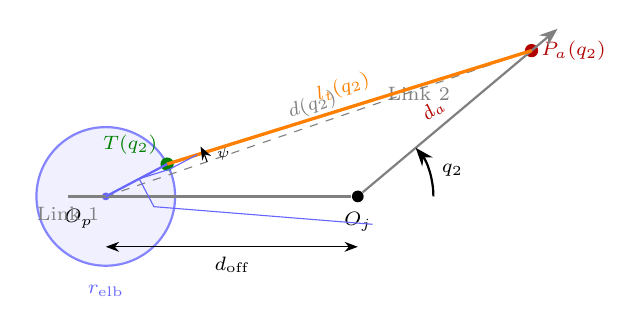
\begin{tikzpicture}[
    >=Stealth, scale=1.6,
    every node/.style={font=\small},
]
    % ── Joint axis ────────────────────────────────
    \node[fill=black, circle, inner sep=1.5pt, label={below:\scriptsize $O_j$}]
        (Oj) at (0,0) {};

    % ── Elbow pulley ─────────────────────────────
    \def\doff{2.0}   % d_off (scaled)
    \def\relb{0.55}  % r_elb (scaled)
    \coordinate (Op) at (-\doff, 0);
    \draw[blue!50, thick] (Op) circle (\relb);
    \fill[blue!30, opacity=0.2] (Op) circle (\relb);
    \node[fill=blue!60, circle, inner sep=1pt,
          label={[font=\scriptsize]below left:$O_p$}] at (Op) {};

    % ── Anchor on link 2 ─────────────────────────
    \def\da{1.8}    % d_a (scaled)
    \def\qtwo{40}   % q2 in degrees
    \coordinate (Pa) at ({\da*cos(\qtwo)}, {\da*sin(\qtwo)});
    \fill[red!70!black] (Pa) circle (1.5pt);
    \node[right, font=\scriptsize, text=red!70!black] at (Pa) {$P_a(q_2)$};

    % ── Link 2 direction ─────────────────────────
    \draw[gray, thick, ->] (Oj) -- ++({\da*1.15*cos(\qtwo)}, {\da*1.15*sin(\qtwo)})
        node[midway, above left, font=\scriptsize] {Link 2};
    \draw[gray, thick] (Oj) -- ++(-2.3, 0) node[below, font=\scriptsize] {Link 1};

    % ── q2 arc ────────────────────────────────────
    \draw[->, thick] (0.6,0) arc[start angle=0, end angle=\qtwo, radius=0.6]
        node[midway, right, font=\scriptsize, xshift=1pt] {$q_2$};

    % ── Distance d(q2) ───────────────────────────
    \draw[dashed, gray] (Op) -- (Pa)
        node[midway, above, sloped, font=\scriptsize] {$d(q_2)$};

    % ── Tangent point T ──────────────────────────
    % Compute tangent angle: phi = atan2(sin,cos) from Op to Pa
    % phi direction from Op to Pa:
    %   Pa - Op = (da*cos(q2)+doff, da*sin(q2))
    % For drawing, approximate the tangent point:
    \pgfmathsetmacro{\dx}{\da*cos(\qtwo)+\doff}
    \pgfmathsetmacro{\dy}{\da*sin(\qtwo)}
    \pgfmathsetmacro{\dist}{sqrt(\dx*\dx+\dy*\dy)}
    \pgfmathsetmacro{\phid}{atan2(\dy,\dx)}
    \pgfmathsetmacro{\psid}{asin(\relb/\dist)}
    \pgfmathsetmacro{\tang}{\phid+\psid}
    \coordinate (T) at ({-\doff+\relb*cos(\tang)}, {\relb*sin(\tang)});
    \fill[green!50!black] (T) circle (1.5pt);
    \node[above left, font=\scriptsize, text=green!50!black] at (T) {$T(q_2)$};

    % ── Tangent line T → Pa ──────────────────────
    \draw[orange, very thick] (T) -- (Pa)
        node[midway, above, sloped, font=\scriptsize] {$l_t(q_2)$};

    % ── Radius to T (perpendicular marker) ───────
    \draw[blue!60, thick] (Op) -- (T);
    \draw[blue!60] ($(T)!2.5mm!(Op)$) -- ++($(T)!2.5mm!90:(Op)-(T)$) -- ($(T)!2.5mm!90:(Op)-(T)$);
    % right angle mark
    \coordinate (rmark1) at ($(T)!2.5mm!(Op)$);
    \coordinate (rmark2) at ($(T)!2.5mm!(Pa)$);
    \draw[blue!60, thin] (rmark1) -- ++($(rmark2)-(T)$) -- (rmark2);

    % ── Angle psi ─────────────────────────────────
    \pgfmathsetmacro{\arcstart}{\phid}
    \pgfmathsetmacro{\arcend}{\phid+\psid}
    \draw[->, thin] ([shift=({\arcstart}:0.85cm)] Op)
        arc[start angle=\arcstart, end angle=\arcend, radius=0.85cm]
        node[midway, right, font=\tiny, xshift=1pt] {$\psi$};

    % ── d_off annotation ─────────────────────────
    \draw[<->, thin] (-\doff, -0.4) -- (0, -0.4)
        node[midway, below, font=\scriptsize] {$d_{\text{off}}$};

    % ── r_elb annotation ─────────────────────────
    \node[font=\scriptsize, blue!60] at (-\doff, -0.75) {$r_{\text{elb}}$};

    % ── d_a annotation ────────────────────────────
    \node[font=\scriptsize, red!70!black, rotate=\qtwo, above] at
        ({\da*0.5*cos(\qtwo)}, {\da*0.5*sin(\qtwo)}) {$d_a$};
\end{tikzpicture}
\caption{Tangent geometry for the offset elbow pulley.  The cable exits the
pulley at the tangent point $T(q_2)$ and runs straight to the
anchor $P_a(q_2)$ on link~2.  The straight segment is exactly the tangent
from $P_a$ to the circle $(O_p,\,r_{\text{elb}})$.  Both $T$ and
the tangent length $l_t$ change with~$q_2$.}
\label{fig:tangent-geom}
\end{figure}

\paragraph{Known quantities.}
\begin{itemize}
    \item Pulley centre: $O_p = (-d_{\text{off}},\;0)$, with
          $d_{\text{off}} = 103\;\text{mm}$.
    \item Pulley radius: $r_{\text{elb}} = 32\;\text{mm}$.
    \item Anchor on link~2, at distance~$d_a$ from the joint:
    \[
        P_a(q_2) = d_a\,\bigl(\cos q_2,\;\sin q_2\bigr).
    \]
\end{itemize}

\paragraph{Step 1 --- distance from anchor to pulley centre.}
%
\begin{equation}\label{eq:dist}
    d(q_2) = \lVert P_a - O_p \rVert
    = \sqrt{d_a^2 + d_{\text{off}}^2 + 2\,d_a\,d_{\text{off}}\cos q_2}.
\end{equation}

\paragraph{Step 2 --- tangent contact angle.}
The straight cable segment is the tangent from the external point~$P_a$ to
the circle $(O_p,\,r_{\text{elb}})$.  The radius to the tangent
point~$T$ is perpendicular to the tangent line, giving:
%
\begin{equation}\label{eq:psi}
    \psi(q_2) = \arcsin\!\Bigl(\frac{r_{\text{elb}}}{d(q_2)}\Bigr).
\end{equation}

\paragraph{Step 3 --- tangent length (straight segment).}
By Pythagoras on the right triangle $O_p$--$T$--$P_a$:
%
\begin{equation}\label{eq:lt}
    l_t(q_2) = \sqrt{d(q_2)^2 - r_{\text{elb}}^2\,}.
\end{equation}

\paragraph{Step 4 --- tangent point location.}
Let $\varphi(q_2) = \mathrm{atan2}\!\bigl(d_a \sin q_2,\;
d_a \cos q_2 + d_{\text{off}}\bigr)$ be the bearing from $O_p$ to~$P_a$.
The tangent point on the pulley is:
%
\begin{equation}\label{eq:Tpoint}
    T(q_2) = O_p + r_{\text{elb}}\,
    \bigl(\cos(\varphi + \psi),\;\sin(\varphi + \psi)\bigr),
\end{equation}
%
where the sign of~$\psi$ selects the branch (right vs.\ left cable).
This is exactly the construction used in \texttt{PulleyBase.compute\_tangent()}
in \texttt{cable/pulley.py}.

\paragraph{Step 5 --- wrap arc.}
Let $\varphi_{\text{in}}$ be the bearing at which the cable arrives from the
Link-1 pulley (fixed, independent of~$q_2$).  The wrap angle is:
%
\begin{equation}\label{eq:alpha}
    \alpha(q_2) = \varphi_{\text{in}} - (\varphi(q_2) + \psi(q_2))
    \qquad\text{(mod $2\pi$, taken positive).}
\end{equation}

\paragraph{Step 6 --- total cable length and moment arm.}
Substituting into \eqref{eq:cable-A-exact}:
%
\begin{equation}\label{eq:lc-full}
    \boxed{l_c(q_2)
    = r_{\text{elb}}\,\alpha(q_2)
    + \sqrt{d(q_2)^2 - r_{\text{elb}}^2}}
\end{equation}
%
The effective moment arm is:
%
\begin{equation}\label{eq:lc-prime}
    l_c'(q_2) = \frac{dl_c}{dq_2}
    = r_{\text{elb}}\,\alpha'(q_2)
    + \frac{d(q_2)\,d'(q_2)}{\sqrt{d(q_2)^2 - r_{\text{elb}}^2}},
\end{equation}
%
where $d'(q_2) = -d_a\,d_{\text{off}}\sin q_2 \,/\, d(q_2)$ from
\eqref{eq:dist}.  Both terms depend on~$q_2$: the wrap-rate term
$\alpha'(q_2)$ and the tangent-length rate.

\begin{mdframed}
\textbf{Why the approximation $l_c' \approx r_{\text{elb}}$ works at small
angles.}\;
When $d_{\text{off}} \ll d_a$ (or equivalently $q_2 \to 0$), the
distance~$d$ is nearly constant, $\psi$ barely changes, and the tangent
length changes slowly.  The wrap-arc term $r_{\text{elb}}\,\alpha'$
dominates, and since $\alpha \approx q_2$ for small angles,
$l_c' \approx r_{\text{elb}}$.  At larger angles the second term in
\eqref{eq:lc-prime} grows, and $l_c'$ deviates from the constant
$r_{\text{elb}}$.
\end{mdframed}

% ─────────────────────────────────────────────────────────────────────────────
\subsection{Spring extension and torque}
% ─────────────────────────────────────────────────────────────────────────────

With motor cable displacements $l_{m,R}$ and $l_{m,L}$, the spring
extensions are (positive $q_2$ = CCW):
%
\begin{align}\label{eq:delta_A}
    \delta_R &= l_{m,R} - l_c(q_2), &
    \delta_L &= l_{m,L} + l_c(q_2).
\end{align}
%
Spring force (tension only):
$F_i = \max(k_{\text{exo}}\,\delta_i + b_{\text{exo}}\,\dot{\delta}_i,\; 0)$.

\medskip\noindent
By virtual work, each cable contributes torque through the effective moment
arm $l_c'(q_2)$, giving the net exo torque on the elbow:
%
\begin{equation}\label{eq:tau_A}
    \boxed{\tau_2^{\text{exo,A}} = l_c'(q_2)\,(-F_R + F_L)}
\end{equation}

% ─────────────────────────────────────────────────────────────────────────────
\subsection{Co-contraction: symmetric pull for pure stiffness}
% ─────────────────────────────────────────────────────────────────────────────

When a disturbance is detected ($|\ddot{q}_2| > 50\;\text{rad/s}^2$), the
controller captures $q_2^{\text{nom}}$ (the pre-disturbance angle) and
commands both motors symmetrically with pretension $\Delta l$:
%
\begin{equation}\label{eq:cmd_A}
    l_{m,R} = l_c(q_2^{\text{nom}}) + \Delta l, \qquad
    l_{m,L} = -l_c(q_2^{\text{nom}}) + \Delta l.
\end{equation}
%
Substituting into \eqref{eq:delta_A} and ignoring damping.  Define
$\Delta l_c = l_c(q_2) - l_c(q_2^{\text{nom}})$ as the cable-length change
due to the disturbance:
%
\begin{align}
    F_R &= k_{\text{exo}}\,(-\Delta l_c + \Delta l), &
    F_L &= k_{\text{exo}}\,(+\Delta l_c + \Delta l).
\end{align}
%
Net torque via \eqref{eq:tau_A}:
%
\begin{equation}\label{eq:tau_cocontract_A}
    \tau_2^{\text{exo,A}}
    = l_c'(q_2)\,(-F_R + F_L)
    = \boxed{2\,k_{\text{exo}}\,l_c'(q_2)\,\Delta l_c}
\end{equation}
%
The pretension $\Delta l$ \textbf{cancels} --- it creates stiffness only,
no net torque at $q_2 = q_2^{\text{nom}}$.  Effective stiffness increase
(linearising $\Delta l_c \approx l_c'\,\Delta q$ for small deflections):
%
\begin{equation}\label{eq:keff_A}
    k_{\text{eff}}^{\text{A}} = 2\,k_{\text{exo}}\,\bigl[l_c'(q_2)\bigr]^{2}
\end{equation}
%
This is the \emph{exact} stiffness formula; it varies with~$q_2$ because
$l_c'$ is not constant for an offset pulley.

% ─────────────────────────────────────────────────────────────────────────────
\subsection{Worked example: 30° impact to 45°}
\label{sec:example-A}
% ─────────────────────────────────────────────────────────────────────────────

\noindent
For numerical evaluation we use the first-order approximation
$l_c(q_2) \approx r_{\text{elb}}\,q_2$ and $l_c' \approx r_{\text{elb}}
= 32\;\text{mm}$ (\cref{eq:approx-A}), which is accurate for
$|q_2| < 45°$.

\begin{enumerate}
    \item[\textbf{T$_0$}:] Joint at $q_2 = 30°$.  Exo \textbf{OFF}.
        $F_R = F_L = 0$.

    \item[\textbf{T$_1$}:] Impact deflects joint to $45°$.
        Acceleration spike triggers co-contraction.
        Controller captures $q_2^{\text{nom}} = 30°$.

    \item[\textbf{T$_2$}:] Motors command via \eqref{eq:cmd_A} with
        $l_c(q_2^{\text{nom}}) \approx r_{\text{elb}} \times 0.524 = 0.0168\;\text{m}$:

        $l_{m,R} = 0.0168 + 0.005 = 0.0218\;\text{m}$,\;
        $l_{m,L} = -0.0168 + 0.005 = -0.0118\;\text{m}$.

        Spring extensions at $q_2 = 45°\;(0.785\;\text{rad})$,
        using $l_c(0.785) \approx 0.032 \times 0.785 = 0.0251\;\text{m}$:
        \begin{align*}
            \delta_R &= 0.0218 - 0.0251 = -0.0033\;\text{m}
                \;\Rightarrow\; F_R = 0 \;\text{(slack)}, \\
            \delta_L &= -0.0118 + 0.0251 = +0.0133\;\text{m}
                \;\Rightarrow\; F_L = 2.67\;\text{N}.
        \end{align*}
        Restoring torque (moment arm $l_c' \approx r_{\text{elb}}$):
        $\tau_2^{\text{exo,A}} = 0.032 \times 2.67 = \boxed{+0.085\;\text{N\,m}}$

    \item[\textbf{Note}:] Only the L cable is active --- the R cable went
        slack because $\Delta l = 5\;\text{mm}$ is insufficient for a
        $+15°$ deflection.  If $\Delta l > l_c' \cdot \Delta q
        \approx 8.4\;\text{mm}$, both cables stay taut and the full symmetric
        torque is $0.107\;\text{N\,m}$.

    \item[\textbf{Approximate $k_{\text{eff}}^{\text{A}}$}:]
        From \eqref{eq:keff_A} with $l_c' \approx r_{\text{elb}}$:
        \[
            k_{\text{eff}}^{\text{A}} \approx 2 \times 200 \times 0.032^2
            = \boxed{0.41\;\text{N\,m/rad}}
        \]
\end{enumerate}


% ═════════════════════════════════════════════════════════════════════════════
\section{Method B: Centred Pulley + Encoder Tracking (Chris)}
\label{sec:methodB}
% ═════════════════════════════════════════════════════════════════════════════

Chris Kalogroulis (April 2026) proposed replacing the two offset elbow
pulleys with \textbf{one pulley centred on the elbow joint axis}
($r_{\text{cp}} = r_p = 47.75\;\text{mm}$).

\begin{mdframed}
\textbf{Fundamental operating principle.}\;
Because the exo pulley sits \emph{on} the joint axis, any rotation of~$q_2$
wraps or unwraps cable around it by exactly $r_{\text{cp}}\,\Delta q_2$.
Without active compensation the springs would stretch, producing undesired
restoring forces during normal motion.

\medskip\noindent
The solution is a \textbf{stepper motor with encoder feedback} that
continuously feeds (or retracts) cable at the same rate the joint moves:
%
\begin{itemize}
    \item \textbf{Exo OFF ($\Delta\theta = 0$):}\;
          The servo tracks~$q_2$ so that $\theta_m = q_2$ (right cable) or
          $\theta_m = -q_2$ (left cable).  This keeps each spring at its
          rest length, producing \emph{zero force} regardless of joint
          angle --- the cable is neither slack nor under tension.
    \item \textbf{Exo ON ($\Delta\theta > 0$):}\;
          The controller adds a symmetric angular offset~$\Delta\theta$
          to both motor commands.  Each spring is extended by
          $r_{\text{cp}}\,\Delta\theta$, creating equal-and-opposite
          pretension.  The net torque at equilibrium is zero, but any
          deviation from~$q_2$ produces a restoring torque proportional
          to~$k_{\text{eff}}^{\text{B}}$.
\end{itemize}

\noindent
\textbf{Contrast with Method~A:}\;
Method~A uses springs on offset pulleys: when the exo motors are off the
springs sit at rest \emph{passively} (no encoder needed) because the cable
geometry does not couple joint rotation to spring extension.  In Method~B
the encoder tracking is \textbf{essential} even when no stiffness is
desired --- without it, joint rotation alone would load the springs.
\end{mdframed}

% ─────────────────────────────────────────────────────────────────────────────
\subsection{Exact cable kinematics (no approximation)}
% ─────────────────────────────────────────────────────────────────────────────

\begin{mdframed}
\textbf{Why Method~B requires no geometric approximation.}\;
Apply the same tangent decomposition as Method~A
(\cref{sec:tangent-geometry}), but now with $d_{\text{off}} = 0$ (pulley
centre $O_p \equiv$ joint axis $O_j$).

\begin{enumerate}
\item \textbf{Distance.}\;
      From \eqref{eq:dist} with $d_{\text{off}} = 0$:
      $d(q_2) = d_a$ --- constant for all~$q_2$.

\item \textbf{Straight (tangent) segment.}\;
      From \eqref{eq:lt}:
      $l_t = \sqrt{d_a^2 - r_{\text{cp}}^2}$ --- also constant.
      The tangent point~$T$ and the anchor~$P_a$ rotate
      \emph{together} around $O_p = O_j$, so their separation
      never changes.

\item \textbf{Wrap arc.}\;
      The bearing from $O_p$ to $P_a$ increases at exactly
      $\dot{q}_2$, so the wrap angle changes linearly:
      $\alpha(q_2) = \alpha_0 + q_2$.
\end{enumerate}

\noindent
Combining:
%
\begin{equation}\label{eq:exact-B}
    l_c^B(q_2)
    = \underbrace{r_{\text{cp}}\,(\alpha_0 + q_2)}_{\text{wrap arc}}
    + \underbrace{\sqrt{d_a^2 - r_{\text{cp}}^2}}_{\text{straight segment (constant)}}
\end{equation}
%
Everything except the $r_{\text{cp}}\,q_2$ term is constant, so the
\emph{change} in cable length is:
%
\begin{equation}\label{eq:delta-lB}
    \Delta l_c^B = r_{\text{cp}}\,\Delta q_2
    \qquad\Longrightarrow\qquad
    (l_c^B)'= r_{\text{cp}}
    \qquad\textbf{(exact, constant for all }q_2\textbf{)}
\end{equation}
%
Contrast with Method~A: the offset ($d_{\text{off}} \neq 0$) makes
$d(q_2)$ vary, so both the straight segment \emph{and} the wrap rate
depend on~$q_2$.  In Method~B that complication vanishes because
$d_{\text{off}} = 0$.
\end{mdframed}

% ─────────────────────────────────────────────────────────────────────────────
\subsection{Encoder tracking and stiffness via angular offset}
% ─────────────────────────────────────────────────────────────────────────────

Each stepper motor continuously tracks the joint encoder, feeding cable at
the rate the joint moves:
%
\begin{equation}\label{eq:tracking}
    \theta_{m,R} = q_2 + \Delta\theta, \qquad
    \theta_{m,L} = -q_2 + \Delta\theta.
\end{equation}
%
The $q_2$ term keeps cables taut (zero extension, zero force during free
rotation).  The $\Delta\theta$ term creates symmetric pretension.

\medskip\noindent
\textbf{Deriving the spring extension (eq~\ref{eq:delta_B}) from the general
form (eq~\ref{eq:delta_A}).}\;
The general spring extension for the right cable is
$\delta_R = l_{m,R} - l_c(q_2)$.  Three substitutions turn this into
the angular form:

\begin{enumerate}
\item \textbf{Cable kinematics} (\cref{eq:delta-lB}):\;
      $l_c(q_2) = r_{\text{cp}}\,q_2 + \text{const}$.

\item \textbf{Motor cable output.}\;
      The exo motor drives a pulley of the same radius $r_{\text{cp}}$
      (1:1 ratio), so
      $l_{m,R} = r_{\text{cp}}\,\theta_{m,R} + \text{const}$
      (the same constant, set at assembly so that $\delta = 0$ when
      $\theta_m = q_2$).

\item \textbf{Substitute both into the general form:}
      \[
          \delta_R
          = r_{\text{cp}}\,\theta_{m,R} - r_{\text{cp}}\,q_2
          = r_{\text{cp}}\,(\theta_{m,R} - q_2).
      \]

\item \textbf{Insert encoder-tracking law} (\cref{eq:tracking}),
      $\theta_{m,R} = q_2 + \Delta\theta$:
      \[
          \delta_R
          = r_{\text{cp}}\bigl((q_2 + \Delta\theta) - q_2\bigr)
          = r_{\text{cp}}\,\Delta\theta.
      \]
      The $q_2$ terms cancel --- this is the whole point of encoder
      tracking.  Repeating for the left cable
      ($\theta_{m,L} = -q_2 + \Delta\theta$,
       $\delta_L = l_{m,L} + l_c = r_{\text{cp}}(\theta_{m,L} + q_2)$):
      \[
          \delta_L
          = r_{\text{cp}}\bigl((-q_2 + \Delta\theta) + q_2\bigr)
          = r_{\text{cp}}\,\Delta\theta.
      \]
\end{enumerate}

\noindent
Result:
%
\begin{align}\label{eq:delta_B}
    \delta_R = r_{\text{cp}}\,\Delta\theta, \qquad
    \delta_L = r_{\text{cp}}\,\Delta\theta
    \qquad\text{(independent of $q_2$)}.
\end{align}
%
Because the tracking is exact (\cref{eq:exact-B}), the motor compensates
$r_{\text{cp}}\,q_2$ of cable per radian with \emph{zero} geometric error,
and any residual torque during free rotation is exactly zero.

% ─────────────────────────────────────────────────────────────────────────────
\subsection{Disturbance response}
% ─────────────────────────────────────────────────────────────────────────────

When a disturbance pushes the joint from $q_2^{\text{nom}}$ to
$q_2^{\text{nom}} + \Delta q$ before the stepper catches up:
%
\begin{align}
    F_R &= k_{\text{exo}}\,r_{\text{cp}}\,(\Delta\theta - \Delta q), &
    F_L &= k_{\text{exo}}\,r_{\text{cp}}\,(\Delta\theta + \Delta q).
\end{align}
%
Net torque (moment arm~$= r_{\text{cp}}$):
%
\begin{equation}\label{eq:tau_B}
    \tau_2^{\text{exo,B}}
    = r_{\text{cp}}\,(-F_R + F_L)
    = \boxed{2\,k_{\text{exo}}\,r_{\text{cp}}^2\,\Delta q}
\end{equation}
%
Same structure as Method~A (\cref{eq:tau_cocontract_A}), but
$r_{\text{cp}}$ replaces $r_{\text{elb}}$.  Effective stiffness increase:
%
\begin{equation}\label{eq:keff_B}
    k_{\text{eff}}^{\text{B}} = 2\,k_{\text{exo}}\,r_{\text{cp}}^2
    = 2 \times 200 \times 0.04775^2
    = \boxed{0.91\;\text{N\,m/rad}}
\end{equation}

% ─────────────────────────────────────────────────────────────────────────────
\subsection{Worked example: same 30° impact to 45°}
\label{sec:example-B}
% ─────────────────────────────────────────────────────────────────────────────

\begin{enumerate}
    \item[\textbf{T$_0$}:] Joint at $q_2 = 30°$.  Stepper tracking
        encoder: $\theta_{m,R} = 0.524 + 0.15 = 0.674\;\text{rad}$.
        Both springs pretensioned by
        $r_{\text{cp}} \cdot \Delta\theta = 7.16\;\text{mm}$.

    \item[\textbf{T$_1$}:] Impact deflects joint to $45°$.
        Stepper still at $\theta_{m,R} = 0.674\;\text{rad}$.

    \item[\textbf{T$_2$}:] Spring extensions:
        \begin{align*}
            \delta_R &= 0.04775 \times (0.674 - 0.785)
                = -0.00534\;\text{m}
                \;\Rightarrow\; F_R = 0 \;\text{(slack)}, \\
            \delta_L &= 0.04775 \times (-0.524+0.15+0.785)
                = +0.01963\;\text{m}
                \;\Rightarrow\; F_L = 3.93\;\text{N}.
        \end{align*}
        Restoring torque:
        $\tau_2^{\text{exo,B}} = 0.04775 \times 3.93 = \boxed{+0.188\;\text{N\,m}}$

        \textbf{2.2$\times$ more restoring torque} than Method~A.

    \item[\textbf{T$_3$}:] Stepper catches up ($\sim\!5\;\text{ms}$),
        re-centres around $q_2^{\text{nom}} = 30°$ with offset $\Delta\theta$.
        Both cables taut; full symmetric stiffness:
        $\tau = 0.91 \times 0.262 = 0.239\;\text{N\,m}$.
\end{enumerate}


% ═════════════════════════════════════════════════════════════════════════════
\section{Comparison of Both Methods}
\label{sec:comparison}
% ═════════════════════════════════════════════════════════════════════════════

% ── Stiffness ratio ──────────────────────────────────────────────────────────
\begin{mdframed}
\textbf{Stiffness ratio (at moderate angles).}\;
Using the first-order approximation $l_c' \approx r_{\text{elb}}$:
$r_{\text{cp}}/r_{\text{elb}} = 47.75/32 = 1.49\times$.
Because stiffness scales as the moment arm squared:
\[
    \frac{k_{\text{eff}}^{\text{B}}}{k_{\text{eff}}^{\text{A}}}
    \approx \frac{r_{\text{cp}}^2}{r_{\text{elb}}^2}
    = \left(\frac{47.75}{32}\right)^{\!2}
    = 2.23\times
\]
Method~B provides more than \textbf{twice} the effective stiffness for the
same spring constant, because $r_{\text{cp}} > l_c'$ for all~$q_2$.
\end{mdframed}

% ── Side-by-side routing comparison TikZ ─────────────────────────────────────
\begin{figure}[h]
\centering
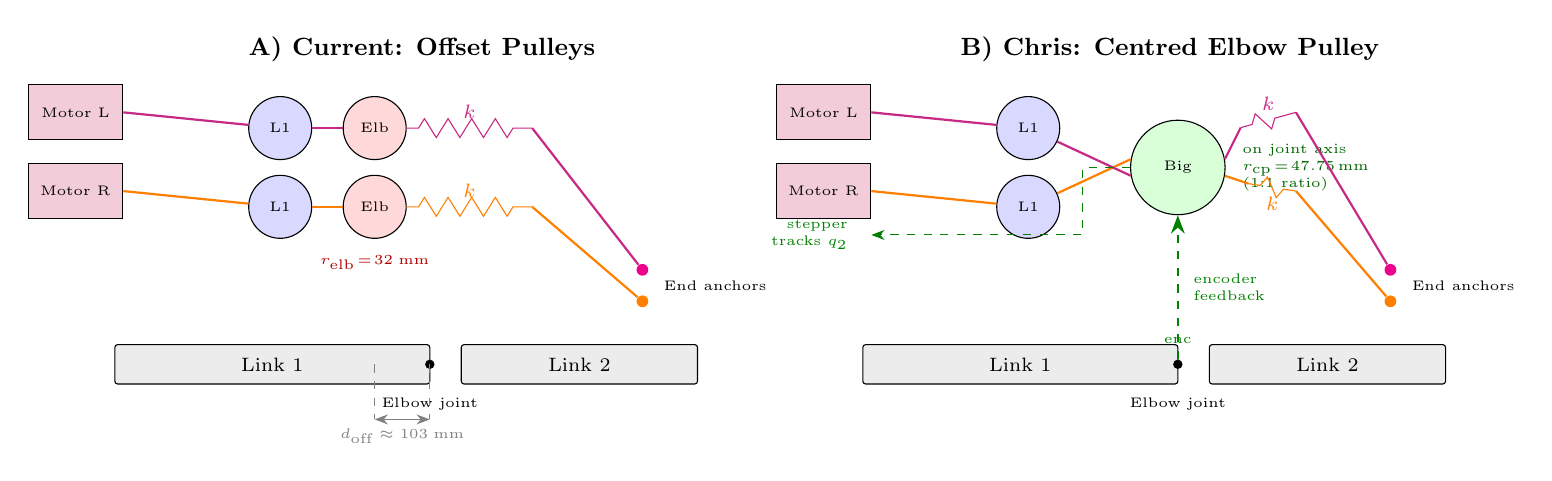
\begin{tikzpicture}[
    >=Stealth,
    pulley/.style={circle, draw, fill=blue!15, minimum size=8mm,
                   font=\scriptsize},
    motor/.style={rectangle, draw, fill=purple!20, minimum width=12mm,
                  minimum height=7mm, font=\scriptsize},
    spring/.style={decorate, decoration={zigzag, segment length=3mm,
                   amplitude=1.2mm, pre length=1.5mm, post length=1.5mm}},
    cable/.style={thick},
    link/.style={draw, fill=gray!15, minimum height=5mm, rounded corners=1pt,
                 font=\scriptsize},
    joint/.style={fill=black, circle, inner sep=1.2pt},
    lbl/.style={font=\scriptsize},
]

% ═══════════════════════════════════════════════════════════════════════════
%  LEFT: Current design (offset pulleys)
% ═══════════════════════════════════════════════════════════════════════════
\begin{scope}[shift={(0,0)}]
    \node[font=\small\bfseries] at (2.2,4.0) {A) Current: Offset Pulleys};

    \node[link, minimum width=40mm] (L1a) at (0.3,0) {Link 1};
    \node[link, minimum width=30mm] (L2a) at (4.2,0) {Link 2};
    \node[joint] (Ja) at (2.3,0) {};
    \node[below, font=\tiny] at (2.3,-0.3) {Elbow joint};

    \node[motor] (MRa) at (-2.2,2.2) {\tiny Motor R};
    \node[motor] (MLa) at (-2.2,3.2) {\tiny Motor L};
    \node[pulley] (P1Ra) at (0.4,2.0) {\tiny L1};
    \node[pulley] (P1La) at (0.4,3.0) {\tiny L1};
    \node[pulley, fill=red!15] (PERa) at (1.6,2.0) {\tiny Elb};
    \node[pulley, fill=red!15] (PELa) at (1.6,3.0) {\tiny Elb};

    \node[circle, fill=orange, inner sep=1.5pt] (ERa) at (5.0,0.8) {};
    \node[circle, fill=magenta, inner sep=1.5pt] (ELa) at (5.0,1.2) {};
    \node[right, font=\tiny] at (5.15,1.0) {End anchors};

    \draw[cable, orange] (MRa.east) -- (P1Ra);
    \draw[cable, orange] (P1Ra) -- (PERa);
    \coordinate (spRa_end) at (3.6,2.0);
    \draw[spring, orange] (PERa.east) -- node[above, lbl] {$k$} (spRa_end);
    \draw[cable, orange] (spRa_end) -- (ERa);

    \draw[cable, magenta!80!black] (MLa.east) -- (P1La);
    \draw[cable, magenta!80!black] (P1La) -- (PELa);
    \coordinate (spLa_end) at (3.6,3.0);
    \draw[spring, magenta!80!black] (PELa.east) -- node[above, lbl] {$k$}
        (spLa_end);
    \draw[cable, magenta!80!black] (spLa_end) -- (ELa);

    \draw[<->, gray, thin] (1.6,-0.7) -- node[below, font=\tiny]
        {$d_{\text{off}} \approx 103\;\text{mm}$} (2.3,-0.7);
    \draw[gray, thin, dashed] (1.6,0) -- (1.6,-0.7);
    \draw[gray, thin, dashed] (2.3,0) -- (2.3,-0.7);
    \node[below, font=\tiny, text=red!70!black] at (1.6,1.5)
        {$r_{\text{elb}}\!=\!32\;\text{mm}$};
\end{scope}

% ═══════════════════════════════════════════════════════════════════════════
%  RIGHT: Chris's suggestion (one centred pulley)
% ═══════════════════════════════════════════════════════════════════════════
\begin{scope}[shift={(9.5,0)}]
    \node[font=\small\bfseries] at (2.2,4.0)
        {B) Chris: Centred Elbow Pulley};

    \node[link, minimum width=40mm] (L1b) at (0.3,0) {Link 1};
    \node[link, minimum width=30mm] (L2b) at (4.2,0) {Link 2};
    \node[joint] (Jb) at (2.3,0) {};
    \node[below, font=\tiny] at (2.3,-0.3) {Elbow joint};

    \node[motor] (MRb) at (-2.2,2.2) {\tiny Motor R};
    \node[motor] (MLb) at (-2.2,3.2) {\tiny Motor L};
    \node[pulley] (P1Rb) at (0.4,2.0) {\tiny L1};
    \node[pulley] (P1Lb) at (0.4,3.0) {\tiny L1};

    \node[pulley, fill=green!15, minimum size=12mm] (PCb) at (2.3,2.5)
        {\tiny Big};
    \node[right, font=\tiny, align=left, text=green!40!black] at (3.0,2.5)
        {on joint axis\\$r_{\text{cp}}\!=\!47.75$\,mm\\(1:1 ratio)};

    \node[font=\tiny, text=green!50!black] at (2.3,0.3) {enc};

    \node[circle, fill=orange, inner sep=1.5pt] (ERb) at (5.0,0.8) {};
    \node[circle, fill=magenta, inner sep=1.5pt] (ELb) at (5.0,1.2) {};
    \node[right, font=\tiny] at (5.15,1.0) {End anchors};

    \draw[cable, orange] (MRb.east) -- (P1Rb);
    \draw[cable, orange] (P1Rb) -- (PCb.170);
    \coordinate (spRb_end) at (3.8, 2.2);
    \draw[cable, orange] (PCb.350) -- ++(0.3,-0.1) coordinate (spRb_start);
    \draw[spring, orange] (spRb_start) -- node[below, lbl] {$k$} (spRb_end);
    \draw[cable, orange] (spRb_end) -- (ERb);

    \draw[cable, magenta!80!black] (MLb.east) -- (P1Lb);
    \draw[cable, magenta!80!black] (P1Lb) -- (PCb.190);
    \coordinate (spLb_end) at (3.8, 3.2);
    \draw[cable, magenta!80!black] (PCb.10) -- ++(0.2,0.4)
        coordinate (spLb_start);
    \draw[spring, magenta!80!black] (spLb_start) --
        node[above, lbl] {$k$} (spLb_end);
    \draw[cable, magenta!80!black] (spLb_end) -- (ELb);

    \draw[->, dashed, green!50!black, thick]
        (Jb.north) -- (PCb.south)
        node[midway, right, font=\tiny, xshift=2pt, align=left]
        {encoder\\feedback};
    \draw[->, dashed, green!50!black]
        (PCb.west) -- ++(-0.6,0) |- ([yshift=-2mm]MRb.south east)
        node[left, font=\tiny, xshift=-5pt, align=right]
        {stepper\\tracks $q_2$};
\end{scope}

\end{tikzpicture}
\caption{Routing comparison.  Both methods share motor pulleys and L1
pulleys.  \textbf{(A)}~Two offset elbow pulleys ($r_{\text{elb}} = 32\;\text{mm}$,
103\,mm before joint); cable payout $l_c(q_2)$ (exact, nonlinear;
$\approx r_{\text{elb}}\,q_2$ at moderate angles).
\textbf{(B)}~One centred elbow pulley ($r_{\text{cp}} = 47.75\;\text{mm}$,
on joint axis); cable payout $= r_{\text{cp}}\,q_2$ (exact).}
\label{fig:routing-comparison}
\end{figure}

% ── Quantitative summary ────────────────────────────────────────────────────
\begin{table}[h]
\centering
\begin{tabular}{@{}lcc@{}}
\toprule
\textbf{Quantity}
    & \textbf{Method A (offset)}
    & \textbf{Method B (centred)} \\
\midrule
Pulley radius
    & $r_{\text{elb}} = 32\;\text{mm}$
    & $r_{\text{cp}} = 47.75\;\text{mm}$ \\[3pt]
Cable kinematics
    & $l_c(q_2)$ (\cref{eq:cable-A-exact})
    & $l = r_{\text{cp}}\,q_2$ (exact) \\[3pt]
Effective stiffness $k_{\text{eff}}$
    & $2\,k_{\text{exo}}\,[l_c']^2$ ($\approx 0.41$ at moderate $q_2$)
    & $0.91\;\text{N\,m/rad}$ \\[3pt]
Restoring torque ($\Delta q = 15°$)
    & $0.085$--$0.107\;\text{N\,m}$
    & $0.188$--$0.239\;\text{N\,m}$ \\[3pt]
Torque during free rotation
    & Small residual (geometry error)
    & Exactly zero \\[3pt]
Cable slack management
    & Passive (springs absorb)
    & Active (stepper tracks encoder) \\[3pt]
Slack risk
    & Low (springs provide compliance)
    & Depends on stepper latency \\
\bottomrule
\end{tabular}
\caption{Quantitative comparison.  Both use $k_{\text{exo}} = 200\;\text{N/m}$.}
\label{tab:force-comparison}
\end{table}

% ── Design trade-offs ────────────────────────────────────────────────────────
\begin{table}[h]
\centering
\begin{tabular}{@{}lll@{}}
\toprule
\textbf{Aspect}
    & \textbf{Method A (offset pulleys)}
    & \textbf{Method B (encoder-tracking)} \\
\midrule
Pulleys per cable
    & 2 (L1 + offset Elbow)
    & 2 (L1 + centred Elbow at joint) \\
Bandwidth requirement
    & Low (slow activation)
    & High (real-time tracking) \\
Single point of failure
    & Springs degrade gracefully
    & Encoder/stepper failure $\to$ slack \\
Prototyping effort
    & Springs + CubeMars
    & Steppers + encoder only \\
Large-angle accuracy
    & Needs lookup table
    & Exact ($r_{\text{cp}} \cdot q_2$) \\
\bottomrule
\end{tabular}
\caption{Design trade-offs between the two routing approaches.}
\label{tab:tradeoff}
\end{table}

% ── Encoder upgrade for Method A ─────────────────────────────────────────────
\subsection{Method A upgrade: adding encoder tracking (A+)}
\label{sec:encoder-upgrade}

Method~A can also use the encoder.  The motor commands track the
exact cable-length function from \eqref{eq:cable-A-exact}:
%
\begin{equation}\label{eq:encoder-A}
    l_{m,R}(t) = l_c\bigl(q_2(t)\bigr) + \Delta l, \qquad
    l_{m,L}(t) = -l_c\bigl(q_2(t)\bigr) + \Delta l.
\end{equation}
%
This keeps both cables taut at all times (no more single-cable slack),
enables always-on variable stiffness, and eliminates the activation
threshold.  On a real-time controller, $l_c(q_2)$ is evaluated via a
lookup table from the tangent-geometry code in
\texttt{cable\_with\_exo\_springs.py}; the approximation
$l_c \approx r_{\text{elb}}\,q_2$ (\cref{eq:approx-A}) may be used for
moderate angles.

% ── Three-mode comparison ────────────────────────────────────────────────────
\begin{table}[h]
\centering
\small
\begin{tabular}{@{}lccc@{}}
\toprule
& \textbf{A: Offset,}
& \textbf{A+: Offset,}
& \textbf{B: Centred,} \\
& \textbf{no encoder}
& \textbf{with encoder}
& \textbf{with encoder} \\
\midrule
Motor command
    & Fixed $l_m$ (on trigger)
    & $l_c(q_2(t)) + \Delta l$
    & $r_{\text{cp}} \cdot q_2(t) + r_{\text{cp}} \cdot \Delta\theta$ \\[3pt]
Cables taut?
    & One may go slack
    & Both (if $\Delta l$ sufficient)
    & Both (if $\Delta\theta$ sufficient) \\[3pt]
Stiffness
    & $0$--$0.41\;\text{N\,m/rad}$
    & $0.41\;\text{N\,m/rad}$
    & $0.91\;\text{N\,m/rad}$ \\[3pt]
Activation
    & Threshold
    & Always on
    & Always on \\[3pt]
Geometric accuracy
    & N/A
    & $l_c(q_2)$ lookup table
    & Exact \\
\bottomrule
\end{tabular}
\caption{Three operating modes.  ``A+'' combines springs with encoder feedback.}
\label{tab:three-modes}
\end{table}

\begin{mdframed}
\textbf{Bottom line.}\;
In Method~B the encoder is \textbf{essential} (cables go slack without it).
In Method~A it is an \textbf{upgrade} that eliminates single-cable slack and
enables always-on variable stiffness.  The trade-off: mechanical simplicity
(Method~B, exact $r \cdot q_2$) versus robustness (Method~A+, springs catch
errors, but need a lookup table for large angles).
\end{mdframed}

\begin{mdframed}
\textbf{Prototype strategy (Chris):}
Build a quick first exosuit with \emph{only} stepper motors and encoder
--- no springs, no CubeMars.  If steppers track the encoder with
$<5\;\text{ms}$ lag, the full system is viable.
\end{mdframed}


% ═════════════════════════════════════════════════════════════════════════════
\section{Dynamics and Control Summary}
\label{sec:dynamics}
% ═════════════════════════════════════════════════════════════════════════════

Full elbow dynamics with both cable systems:
%
\begin{equation}\label{eq:full}
    M_{22}\,\ddot{q}_2 + c_2(\bq,\dot{\bq}) + g_2(\bq)
    = \underbrace{r_p\,(T_{\text{green}} - T_{\text{red}})}_{\text{drive cables}}
    \;+\;
    \underbrace{r_{\text{eff}}(q_2)\,(-F_R + F_L)}_{\text{exo cables (when active)}}
\end{equation}
%
where the effective moment arm is
$r_{\text{eff}} = l_c'(q_2)$ (Method~A, varies with~$q_2$) or
$r_{\text{eff}} = r_{\text{cp}}$ (Method~B, constant).

\begin{figure}[h]
\centering
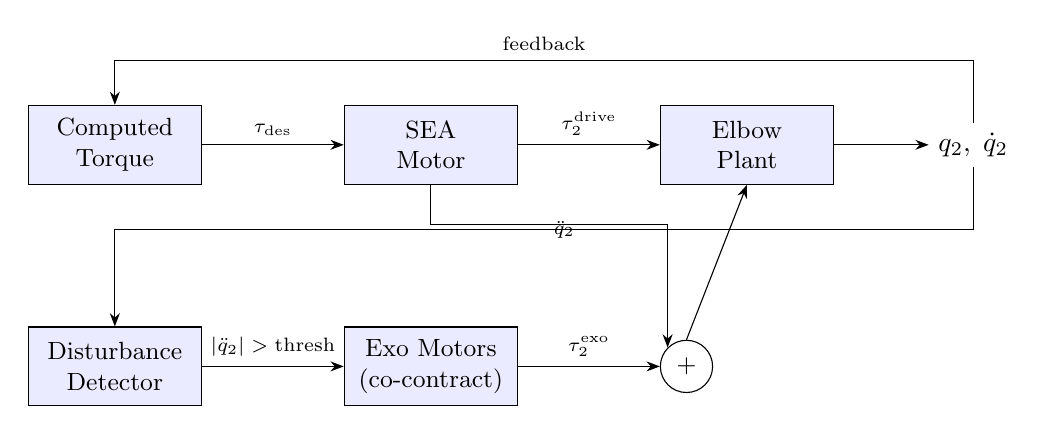
\begin{tikzpicture}[
    >=Stealth,
    block/.style={rectangle, draw, fill=blue!8, minimum width=22mm,
                  minimum height=10mm, font=\small, align=center},
    sum/.style={circle, draw, minimum size=6mm, font=\small},
    node distance=14mm and 18mm,
]
    \node[block] (ct) {Computed\\Torque};
    \node[block, right=of ct] (sea) {SEA\\Motor};
    \node[block, right=of sea] (plant) {Elbow\\Plant};
    \node[right=12mm of plant] (q2) {$q_2,\;\dot{q}_2$};

    \draw[->] (ct) -- node[above, font=\scriptsize] {$\tau_{\text{des}}$} (sea);
    \draw[->] (sea) -- node[above, font=\scriptsize] {$\tau_2^{\text{drive}}$} (plant);
    \draw[->] (plant) -- (q2);

    \node[block, below=18mm of ct] (detect) {Disturbance\\Detector};
    \node[block, right=of detect] (exo) {Exo Motors\\(co-contract)};
    \node[sum, right=of exo] (sum) {$+$};

    \draw[->] (q2.south) -- ++(0,-0.8) -| (detect.north)
         node[near start, right, font=\scriptsize] {$\ddot{q}_2$};
    \draw[->] (detect) -- node[above, font=\scriptsize]
         {$|\ddot{q}_2|>\text{thresh}$} (exo);
    \draw[->] (exo) -- node[above, font=\scriptsize]
         {$\tau_2^{\text{exo}}$} (sum);
    \draw[->] (sum.north) -- (plant.south);
    \draw[->] (sea.south) -- ++(0,-0.5) -| (sum.north west);
    \draw[->] (q2.north) -- ++(0,0.8) -| (ct.north)
         node[near start, above, font=\scriptsize] {feedback};
\end{tikzpicture}
\caption{Control block diagram.  Drive path (top) runs continuously;
exo path (bottom) activates on disturbance detection.}
\label{fig:control}
\end{figure}

\begin{table}[h]
\centering
\begin{tabular}{@{}lll@{}}
\toprule
\textbf{Aspect} & \textbf{Biological} & \textbf{Our mechanism} \\
\midrule
Agonist/Antagonist  & Biceps/Triceps         & Drive green/red cables \\
Co-contraction      & Both muscles activate  & Both exo motors pull \\
Stiffness source    & Muscle short-range stiffness & Exo spring $k_{\text{exo}}$ \\
Activation trigger  & Reflex (stretch reflex) & $|\ddot{q}_2| > $ threshold \\
Decoupling          & Reciprocal inhibition   & Spring at rest $\Rightarrow F=0$ \\
\bottomrule
\end{tabular}
\caption{Biological co-contraction analogy.}
\label{tab:bio}
\end{table}

\end{document}
